% Chapter 1

\chapter{Absolute power calibration} % Main chapter title
\label{Chapter5} % For referencing the chapter elsewhere, use \ref{Chapter1} 
This chapter describe the absolute power calibration procedure of KAGRA photon calibrator.
The systematic error of the absolute power is most largest in LIGO.
They measure the laser power with integrating sphere and InGaAs photodetector because displacement of mirror corresponds to laser power. 
The absolute power injected to the ETM can be obtained as average of input power at Tx module and the output power at Rx module as follows:
\begin{equation}
P=\frac{P_{\mathrm{TxPD}}+P_{\mathrm{RxPD}}}{2}=\frac{1+e}{2e}P_{\mathrm{RxPD}},
\end{equation}
where $P_{\mathrm{TxPD}}$ and $P_{\mathrm{RxPD}}$ are the measured power of the transmitter module photo detector(TxPD) and the receiver module photodetector (RxPD), and $e=P_{\mathrm{TxPD}}/P_{\mathrm{RxPD}}$ is optical efficiency.
Therefore, $P_{\mathrm{TxPD}}$ and $P_{\mathrm{RxPD}}$ limit the calibration accuracy of the absolute displacement of the mirror.
To calibrate $P_{\mathrm{TxPD}}$ and $P_{\mathrm{RxPD}}$, we employ the working standard (WS) and the gold standard (GS). 

The WS of KAGRA (WSK) is the combination of integrating sphere and InGaAs photo detector (see Fig.~\ref{fig:KWS}), which is calibrated against GS of LIGO (GSL) in LHO lab as calibrated by NIST. LIGO also make working standards for LHO and LLO as shown in Fig~\ref{fig:GS_WS}.
The ratio of measured voltage of WS and GS detectors are obtained as
\begin{equation}
\frac{V_{\mathrm{WSK}}}{V_{\mathrm{GSL}}}.
\end{equation}
We can calibrate the response of WS using GS through this equation.

We will also use the WSK to calibrate the TxPD and RxPD, which are inside the Tx module and Rx module of Pcal, respectively. We will measure the ratio of voltage of TxPD and RxPD as follows
\begin{equation}
\frac{V_{\mathrm{TxPD}}}{V_{\mathrm{KWS}}}.
\end{equation}

Finally,  we obtain the calibration power $P_{\mathrm{GW}}$ using the power standard laser in NIST.
Then, we can get the calibrated $P_{\mathrm{TxPD}}$ and $P_{\mathrm{RxPD}}$ as follows:

\begin{eqnarray}
P_{\mathrm{TxPD}}=\frac{V_{\mathrm{TxPD}}}{V_{\mathrm{KWS}}}\frac{V_{\mathrm{WSK}}}{V_{\mathrm{GSL}}}P_{\mathrm{GS}}, \\
P_{\mathrm{RxPD}}=\frac{V_{\mathrm{RxPD}}}{V_{\mathrm{KWS}}}\frac{V_{\mathrm{WSK}}}{V_{\mathrm{GSL}}}P_{\mathrm{GS}}
\end{eqnarray}

\begin{figure}
\begin{center}
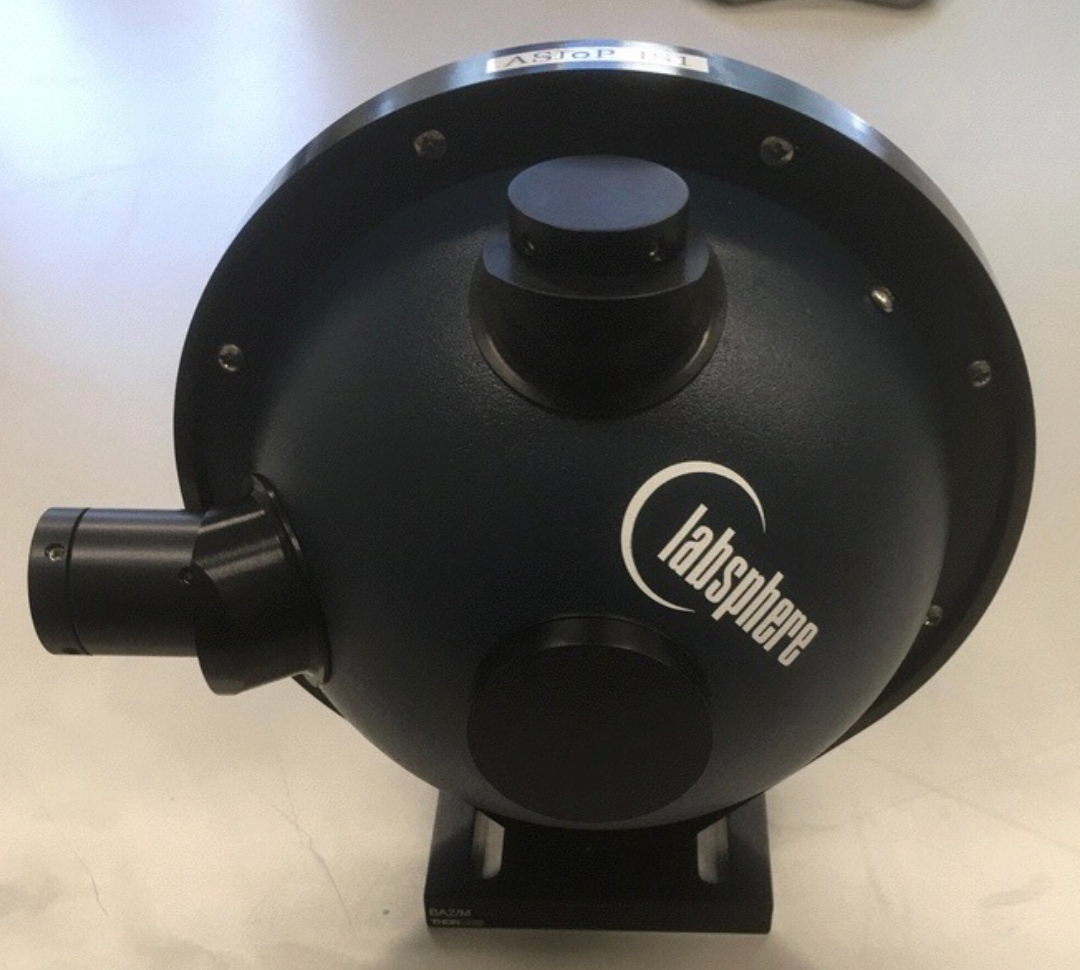
\includegraphics[width=14cm]{Figures/KWS.eps}
\caption{KAGRA working standard.} 
\label{fig:KWS} 
\end{center}
\end{figure}

\begin{figure}
\begin{center}
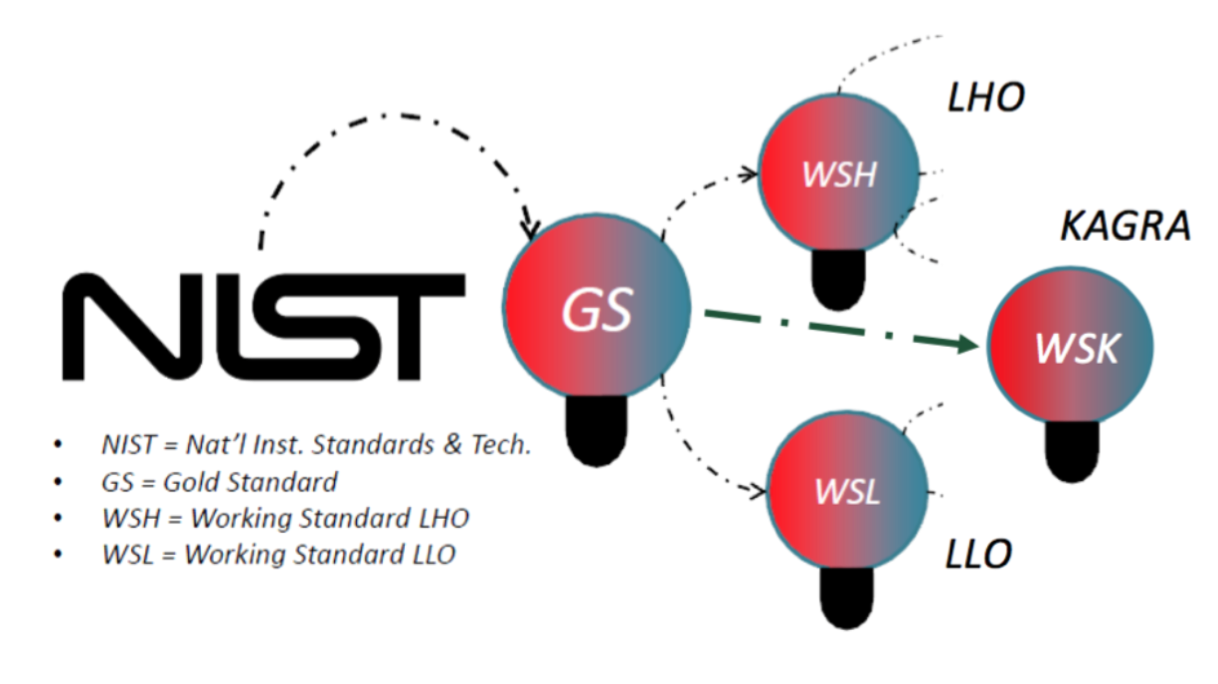
\includegraphics[width=14cm]{Figures/GS_WS.eps}
\caption{comparison with GS and WS.} 
\label{fig:GS_WS} 
\end{center}
\end{figure}

\section{Calibration in LHO}
We explain the calibration of WSK in LIGO.
To avoid systematic error of localization from GS, we need to calibrate the displacement of mirror by each interferometer. LIGO use the GSL calibrated by NIST for calibration of absolute power of LLO and LHO.
We also calibrate WSK using same GSL.
To accurate measurement, we bring the WSK, photo detector and voltmeter to LHO.

We employ  the four inch integrating sphere made by Labsphere. The model number of the integrating sphere is 3P-LPM-040-SL. We mount the photo detector at the top of integrating sphere.
The detail of photo detector is written at Sec.~\ref{PD}.
The voltmeter is make by Keithley company as shown in Fig.~ref{fig:Keithley}. The model number of voltmeter is 2100/100. To reduce the instrumental bias, we fix the pair of voltmeter and WS. 

We check the time trend of the optical efficiency, $V_{\mathrm{GS}}/V_{\mathrm{WS}}$ by 4 month.
\begin{figure}
\begin{center}
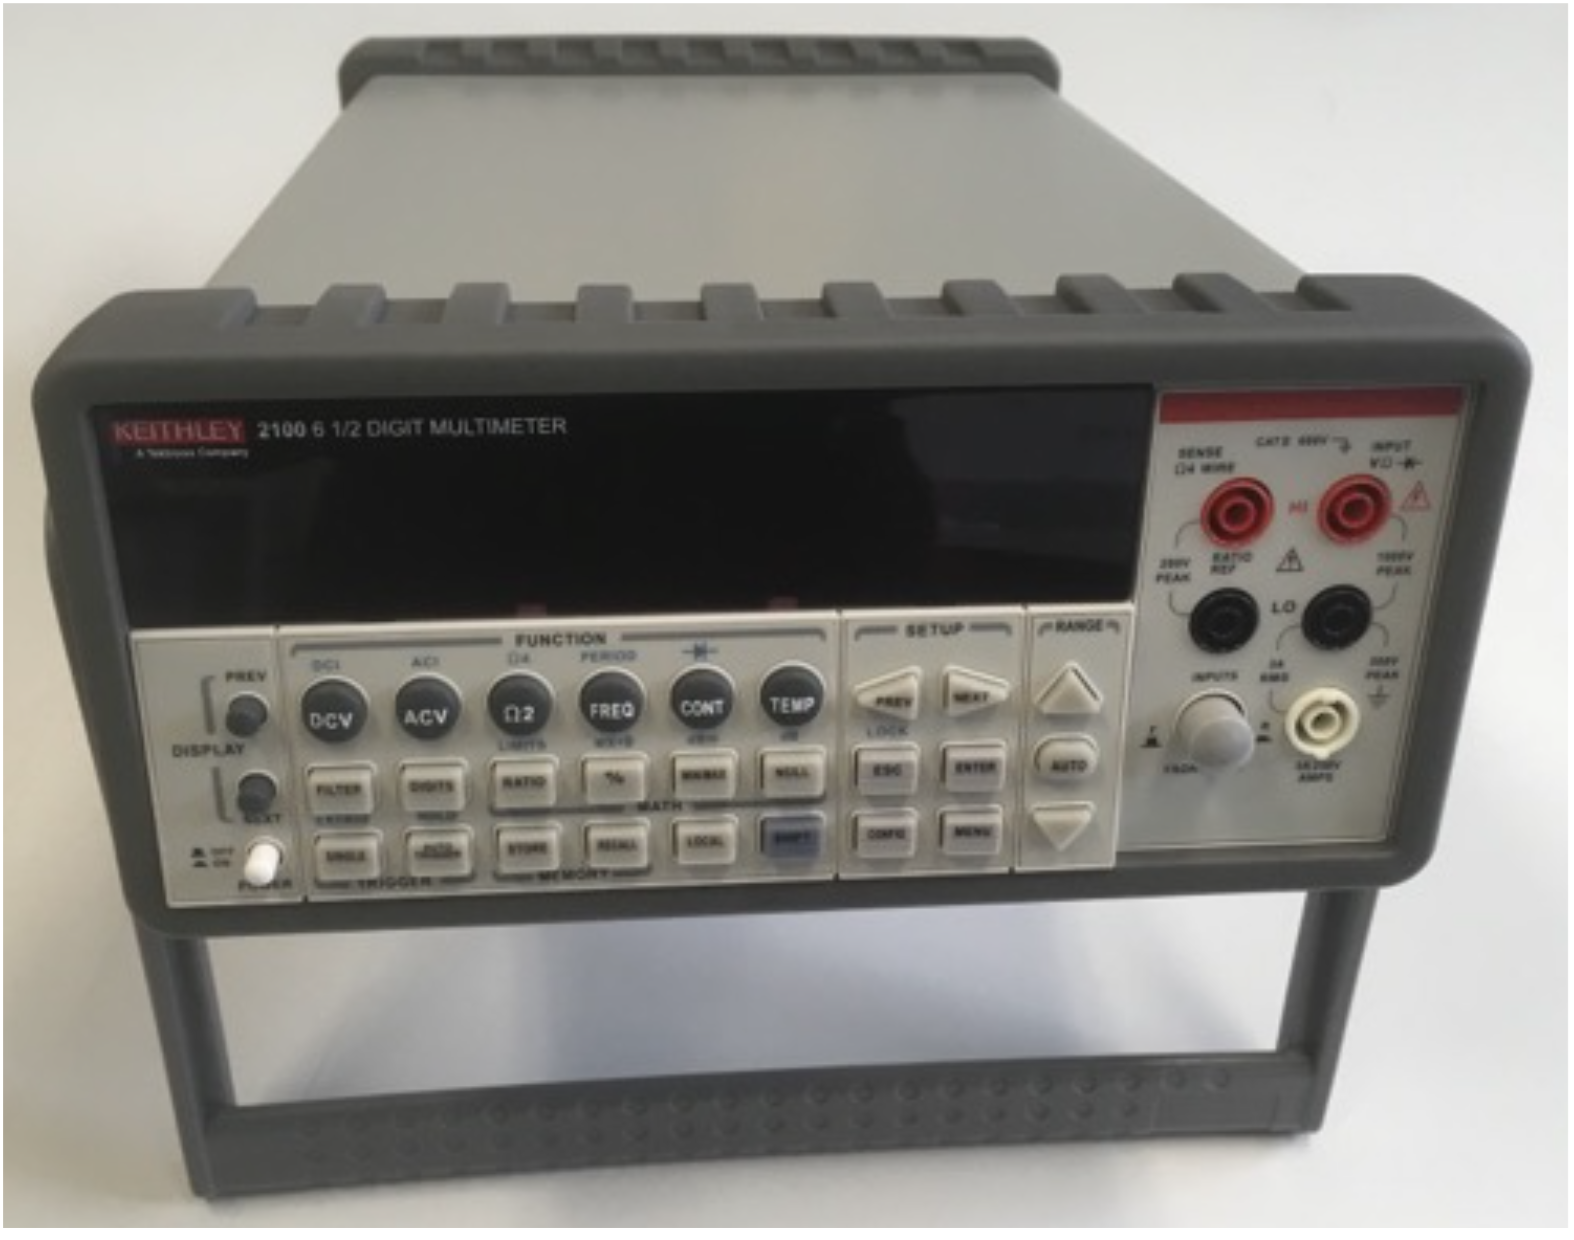
\includegraphics[width=14cm]{Figures/Keithlay.eps}
\caption{Voltmeter made by keithlay.} 
\label{fig:Keithley} 
\end{center}
\end{figure}
%-------------------------------
\section{Calibration in end-station}
We calibrate the TxPD and RxPD in X/Y end station every month. When we calibrate the TxPD, we open the side box and mount the WSK as shown in Fig~\ref{fig:WSK_end_station}. We measure the power of two beams. We calculate the ratio between TxPD and sum of two beam voltage measured by WSK. 


\begin{figure}
\begin{center}
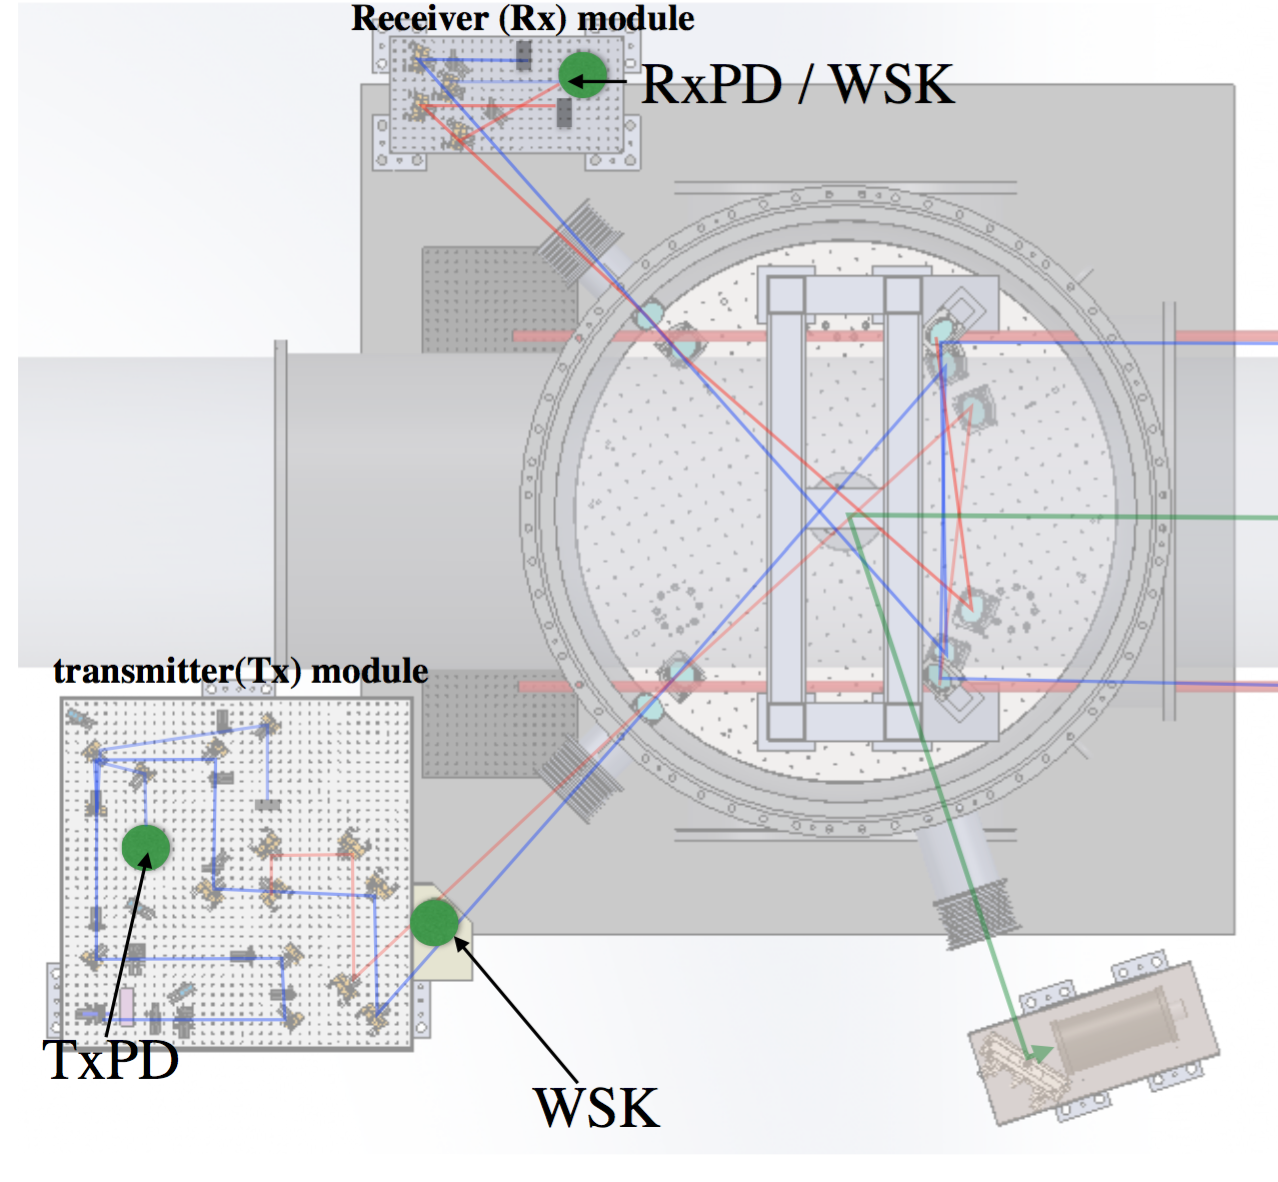
\includegraphics[width=14cm]{Figures/WSK_end_station.eps}
\caption{Calibration of end-station. We calibrate TxPD and RxPD using WSK.} 
\label{fig:WSK_end_station} 
\end{center}
\end{figure}

We also calibrate the RxPD. We replace from RxPD to WS and measure the ratio of the voltages. 

We check the time trend of the optical efficiency, $V_{\mathrm{TxPD}}/V_{\mathrm{WS}}$, $V_{\mathrm{RxPD}}/V_{\mathrm{WS}}$, by 1 month.

Furthermore, we monitor the time trend of $V_{\mathrm{TxPD}/V_{\mathrm{RxPD}}}$, everyday.

If we find unstable region in time trend, we need to propagate the uncertainty as the systematic error.

\section{KAGRA Gold Standard}
Photo-detectors used in the transmitter and receiver modules to measure absolute laser power should be calibrated by laser power standard system. The Gold Standard of LIGO (GSL) is calibrated in NIST in US every year. A new test bench to calibrate LIGO PCal photo-detectors were developed in NIST since LIGO PCal uses unpopular wavelength laser of 1047nm to avoid to couple with main laser beam of interferometer with 1064nm in wavelength with keeping sufficient transmittance and reflectivity of optics. Finally, uncertainty of absolute laser power is mainly coming from uncertainty of the standard in NIST. 

In fact, absolute laser power is one of the worst precision items in the field of standard. Fig.~\ref{fig:Power_standard} shows performance comparison of laser power standard system in national standard institutions in the world, reported in 2009~\cite{EUROMET}. There is large inconsistency of about 4\% among the institutions. Rare cross-check of laser power standard among institutions carries out. In future work, we are planning to introduce new test bench of laser power standard with 1047nm in wavelength in AIST(National Institute of Advanced Industrial Science and Technology)  in Japan. We have already started discussion of such test bench development with a scientist in AIST. We newly make the Gold standard of KAGRA (GSK) using the integrating sphere with photo detector. By comparison with laser power standards both in NIST and AIST, and also with GSL and GSK themselves between aLIGO and KAGRA, we evaluate systematic errors of PCals, and achieve to improve its accuracy. To calibrate the WSK, we plan to make a optical bench in Toyama university as shown in Fig.~\ref{fig:Toyama}. We will bring and compare the calibrated WSK and GSL in LHO.

\begin{figure}
\begin{center}
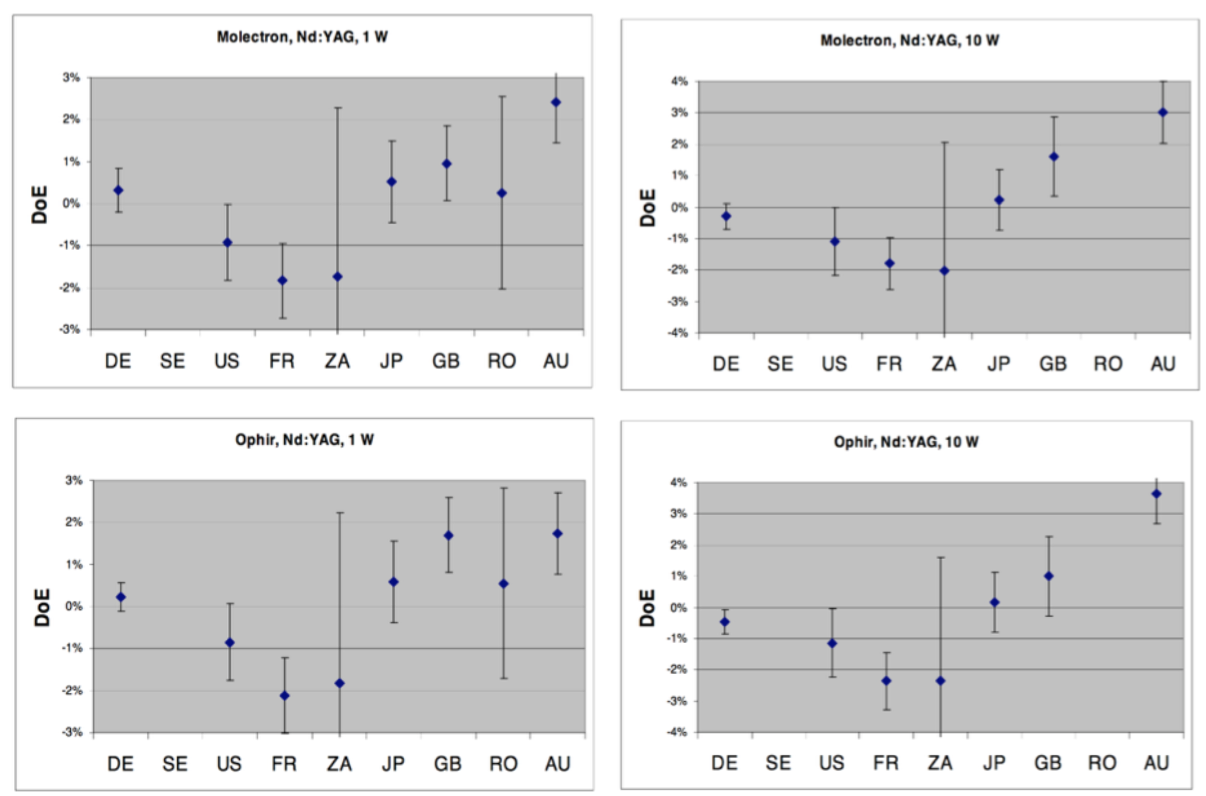
\includegraphics[width=14cm]{Figures/Power_standard.eps}
\caption{
Performance comparison of laser power standard system at 1064nm wavelength and 1W power in the national standard institutions in the world~\cite{EUROMET}.
} 
\label{fig:Power_standard} 
\end{center}
\end{figure}

\begin{figure}
\begin{center}
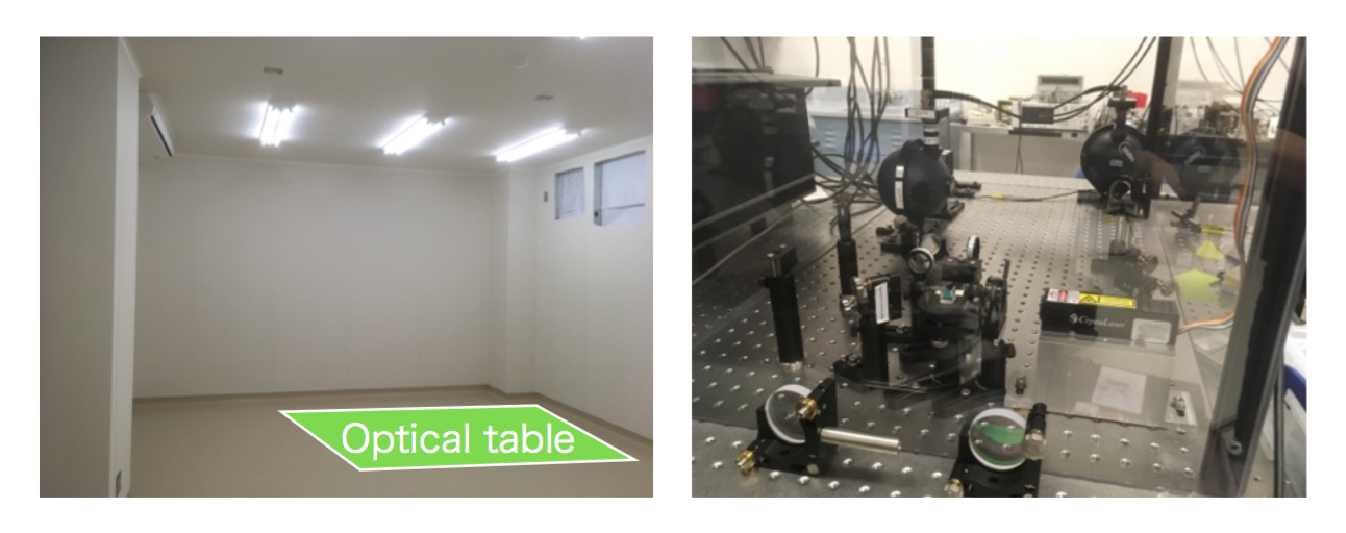
\includegraphics[width=14cm]{Figures/Toyama.eps}
\caption{.} 
\label{fig:Toyama} 
\end{center}
\end{figure}

\section{Summary}
This chapter has considered the absolute power calibration for KAGRA Pcal. The uncertainty of the displacement of ETM is corresponding to that of the absolute power of PCal laser. We will monitor the trend of each parameter because it propagate to the systematic error of h(t). 






